\documentclass[10pt,a4paper]{article}
\usepackage[utf8]{inputenc}
\usepackage[slovak]{babel}
\usepackage[IL2]{fontenc}
\usepackage{amsmath}
\usepackage{amsfonts}
\usepackage{amssymb}
\usepackage{graphicx}
\begin{document}

\centerline{\Huge \bf Reinforcement leraning - Dots and Boxes}

\section*{Abstrakt}
Dots and Boxes je jednoduchá hra pre dvoch hráčov, ktorá sa hrá na štvorcovej mriežke.
V tejto práci aplikujeme metódy učenia odmenou a trestom na natrénovanie automatického hráča. 
V práci kladieme dôraz najmä na výber vhodnej metódy, prispôsobenie Q-learningu pre našu potrebu, jeho implementáciu.
Prvej časti predstavíme hru Dots and Boxes, v druhej, vysvetlíme náš postup a úvahy.
Druhá časť sa ďalej člení na časti: Uvažované prístupy, kde robíme rozbor možných metód ako sa k problému postaviť,
Implementáciu, kde rozoberieme podrobnosti zvoleného prístupu, Testovanie, kde ukážeme úspešnosť nášho úsilia.



\section{Hra Dots and Boxes}
Túto hru publikoval Édouard Lucas (1989). Hrá sa na štvocovej mriežke, obvykle $4\times 4$ (alebo $6\times 6$) mrežových bodov, kde sú na začiatku vyznačené len mrežové body.
Hráči striedavo dokresľujú hrany mriežky. Ak hráč dokreslenou hranou uzavrie 1x1 štvorček, získava bod (ak uzavrie 2 štvorčeky, získava dva body)
a ťahá ešte raz. Hra končí po dokreslení všetkých hrán, vyhráva hráč, ktorý má viac bodov. V prípade rovnosti bodov vyhráva hráč, ktorý nezačínal. 

\bigskip

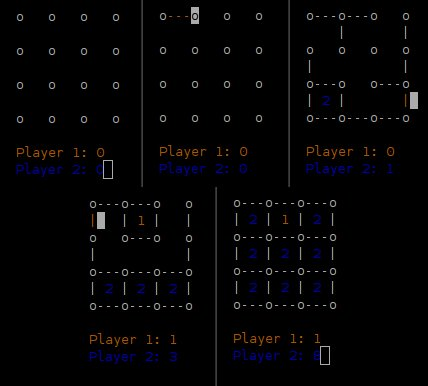
\includegraphics[trim = -40mm 0 0 0, clip, scale=.5]{game1.jpg}

Víťazná stretégia pre túto hru rozhodne existuje, lebo je to hra s úplnou informáciou, bez náhodných prvkov. 
No zhrnúť ju nie je také jednoduché. 



\section{Reinforcement learning}


Celkovo na mriežke $n\times n$ bodov je $n_h = 2n(n-1)$ hrán, t.j. 24 pre $n=4$ 
alebo 60 pre $n=6$. Každá hrana môže byť buď už nakreslená alebo prázdna, to dáva
celkovo $2^{n_h}$ rôznych stavov. V každom stave máme možnosť vybrať si akciu - dokresliť 
niektorú (doteraz prázdnu) hranu. Stredná hodnota počtu akcií je $n_h/2$ 
(lebo počet stavov kde chýba $n_h/2 + k$ hrán je rovnaký ako počet stavov, kde chýba $n_h/2 -k$ hrán, 
jednoduchá bijekcia medzi nimi je invertovanie všetkých hrán).
Čiže celkový priestor dvojíc (stav, akcia) má $$|P| = 2^{n_h}n_h/2 = 2^{2n(n-1)}n(n-1)$$
prvkov. Pre $n=4$ je $|P| > 2^{27}$, pre $n=6$ je $|P| > 2^{65}$.
To je pomerne veľký priestor na prehľadávanie.




\subsection{Uvažované prístupy}


Podľa skúseností pri vytváraní tohto projektu by sme mohli subjektívne rozdeliť uvažované metódy, na 2 typy. 
(Ak mi niekto ukáže novú hru a chce aby som sa ju naučil hrať, tak mám dve možnosti ako k tomu pristúpiť)
\begin{enumerate}
\item Typ mysliteľ (najprv myslým, potom hrám) - sadnem si ku plániku a začnem ju nejako analyzovať, asi 
	asi najlepšie od konca a snažím sa zapamätať si, ktoré pozície sú pre mňa dobré a ktoré nie a potom keď si
	to chce niekto zahrať, snažím sa ťahať do takých pozícii, ktoré sú pre súpera zlé.
\item Typ hráč (najprv hrám, potom myslým) - zahrám si niekoľko skúšobných hier, v ktorých ťahám viacmenej náhodne
	a skúšam sa z nich niečo naučiť. Postupne ako sa učím svoje poznatky uplatnujem pri hraní ďalších skúšobných hier.
\end{enumerate}

Samozrejme existuje aj tretí typ - nejaká kombinácia týchto dvoch.


Pozrime sa na známe metódy: value iteration, Q-learning.


\subsubsection{Value iteration} 
Value iteration je rozhodne mysliteľ. 
Samotná však nepripadá do úvahy (pre $n>4$), lebo opakovane prejsť všetky stavy by trvalo príliš dlho.
a tiež je prakticky nemožné uchovávať kompletnú tabuľku hodnôt pre všetky dvojice (stav, akcia). 

Jedna možnosť ako vytvoriť slušného hráča je napríklad natrénovať value-iteration pre posledných $k$ ťahov a na zvyšok použiť rozumnú heuristiku.



\subsubsection{Q-learning}
Podobné negatíva má aj Q-learning. 

Skúšali sme modelovať funkciu $Q$ pomocou rôznych metód ML. 
Najväčším problémom je voľba správnej metódy. Väčšina metód je navrhnutých tak, aby sa predchádzalo overfitom, čo je v našom prípade trošku problém. 
Jeden zjavný, vynútený, dobrý ťah v okolí samých zlých možno vyzerá v dátach presne ako outlier, resp. chyba 
a väčšina metód ho teda nefitne. 
Takže v úvahe ostávajú asi len neurónové siete a rozhodovacie stromy, lebo tie prinášajú pomerne veľkú voľnosť pri fitovaní.

Druhým veľkým problémom je trénovanie. Ako vstup pre funkciu Q sme použili binárny vektor reprezentujúci aktuálnu hraciu plochu (1 ak je hrana, 0 ak nie je).  
Treánovanie typom hráč je problém, lebo máloktorý model podporuje online-learning (postupné učenie sa po menších kúskoch dát). 
A pri skúšaní tohto prístupu sa veľmi často stávalo, že hodnoty príliš skákali. 
Jedine pri veľmi malých neurónových sieťach to vyzeralo zo začiatku dobre (podarilo sa natrénovať aspoň nejaké správne počiatočné hodnoty), 
ale po väčšom počte hier sa veľa týchto hodnôt zmenilo a teda aj všetko ďalšie updatovanie už bolo takmer nanič. Žiaden slušný výsledok sa mi takto docieliť nepodarilo. Možno by bolo zaujímavé okrem vektoru reprezentujúceho hraciu plochu priložiť nejaké ďalšie predpočítané premenné. Alebo vyskúšať iný spôsob updatovania Q.

Trénovanie typom mysliteľ by trvalo príliš dlho, a hlavne vygenerovať všetky trénovacie príklady naraz, ktoré chceme fitnúť je takmer nemožné.
Celkom rozumné sa zdá byť natrénovať zvlášť každú "vrstvu" $Q_m$, kde pod $m$-tou vrstvou myslíme všetky stavy plochy, kde ostáva práve $m$ nezafarbených hrán. Totiž ak budeme postupovať od konca, tak vieme presne zistiť $Q_0$, z nej $Q_1$, z nej $Q_2$, atď. Toto sme využili na natrénovanie optimálnej hry posledných $k$ ťahov, na túto časť by bolo asi vhodné použiť rozhodovací strom pre každú vrstvu. No hodnoty $Q_m$ by sme museli aj tak najprv zistiť a až potom fitnúť rozhodovacím stromom, keďže tie nepodporujú online learning. Takže jediná výhoda by bola, že natrénovaný strom by zaberal menej miesta v pamäti.




\subsection{Naša implementácia}


Prvá otázka je ako odmeňovať, keďže o tom je učenie odmenou a trestom. Môžeme odmeňovať za každý získaný bod
alebo odmeňovať až na konci za výhru (resp. trestať za prehru).

\subsubsection{Odmena za každý bod}

Pod stavom hry budeme rozumieť stav hracej plochy (bez ohľadu na to, kto je na ťahu a aké je aktuálne skóre), 
lebo len to by malo vplývať na to aký ťah urobí optimálny hráč. 
Je zrejmé, že v každej pozícii je nejaký najlepší ťah (resp. množina najlepších ťahov) a našim cieľom je hľadať práve tieto ťahy. 


Uchovávanie hodnôt (či už Q-funkcie, alebo hodnôt vo value iteration) pre dvojice (stav, akcia) trošku zjednodušiť. 
Ak by sme používali value-iteration alebo Q-learning rovno ako z krabičky, tak nevyužijeme špecifiká, ktoré táto hra ponúka.



Keďže poznáme presne stav, do ktorého posunieme hru po našom ťahu, vieme presne určiť svoju odmenu. Ak by sme za každý získaný bod odmeňovali 
jedným bodom, musíme nechať discount factor = 1. Totiž discount factor teraz nedáva zmysel, lebo hra trvá stále rovnako dlho a skóre, ktoré získame s časom nijako nedegraduje a zbytočne by sme dávali dôraz na ťahy, v ktorých získame políčka skôr, miesto ťahov pri korých získame viac políčok, ale neskôr.

Predstavme si takúto interpretáciu hodnôt. Pre stav $s$ si budeme pamätať 
$$Q(s) = \left[\begin{array}{l}
\mbox{koľko bodov ešte vie hráč na ťahu získať od tohto ťahu do konca,} \\
\mbox{ak my aj súper hráme najlepšie ako sa dá}.
\end{array}\right]$$. 

Teraz vidno, prečo si nemusíme pamatať hodnotu zvlášť pre náš ťah v stave $s$ a zvlášť pre súperov. Totiž ak hráč na ťahu vie získať $Q(s)$ bodov, druhý vie získať všetky ostatné, doteraz nezískané.

Takáto funkcia $Q$ musí splňovať isté vzťahy. Ak som v stave $s$, spravím akciu $a$ a plocha sa ocitne v stave $s_a$, sú dve možnosti:
\begin{enumerate}
\item získal som $R(a)>0$ bodov, takže zo stavu $s_a$ buďem opäť ťahať ja. Vtedy chcem som aby $Q(s_a)+R(a)$ bolo čo najväčšie (aby som celkovo získal čo najviac bodov).
\item získal som $R(a)=0$ bodov, takže v stave $s_a$ bude ťahať súper. Vtedy chcem aby $Q(s_a)$ bolo čo najmenšie (aby som súpera dostal do pozície, v ktorej získa najmenej bodov). Alebo teda z môjho pohľadu, ak on vie získať maximálne $Q(s_a)$ bodov, ja viem získať ešte najmenej všetky ostatné,
chcem teda maximalizovať $pnb(s)-Q(s_a)$, kde $pnb(s):=$[\# nezískaných bodov].
\end{enumerate}
Označme teda $f(s,a)$ funkciu, ktorá spojí tieto dve možnosti a vráti počet bodov, ktoré viem určite získať ak som v stave $s$ a urobím akciu $a$.
$$f(s,a) = \left\lbrace \begin{array}{ll}
Q(s_a)+R(a), & \mbox{ pre } R(a)>0,\\
pnb(s)-Q(s_a) & \mbox { pre } R(a)=0.
\end{array}\right.
$$
Najlepšiu akciu $a_{opt}$ v každom stave $s$ potom vieme určiť ako 
$$ a_{opt} = \mbox{argmax}_{a\in A(s)} f(s,a)$$
Tento vzťah zároveň ponúka spôsob ako určiť $Q(s)$, ak poznáme $Q(s_a)$ pre všetky $a\in A(s).$
Totiž, ak v stave $s$ vieme získať $Q(a)$ bodov a urobíme optimálny ťah, tak spolu s ním vieme vo zvyšku hry získať presne $Q(s)$ bodov, teda 
$$Q(s) = f(s,a_{opt}) = max_{a\in A(s)}f(s,a).$$
Na tomto vzťahu postavíme aj náš update $Q$, s learning rate-om $\lambda$,
$$Q_{new}(s) = Q_{old}(s)+ \lambda(max_{a\in A(s)}f(s,a) - Q_{old}(s)).$$


Výhodou tejto reprezentácie $Q$ je kompaktnosť - nižšie pamäťové nároky, rýchlejšie trénovanie, 
ďalšou výhodou je, že ak ju budeme trénovať pri hraní, tak náš hráč nikdy nebude hlúpnuť. 
Čím viac hier odohrá, tým bude lepší, aj keby hral proti zlým súperom, takže learning rate môže byť kľudne 1.
Nevýhodou je, že teraz musíme počítať hodnotu funkcie $f$. No je to dobrý trade-off, lebo čas na výpočet $f$ pre väčšie $n$ nerastie, 
narozdiel od počtu akcií, pre ktoré by sme si museli pamätať tieto hodnoty.

\paragraph{Ukladanie $Q$.}

Hodnoty $Q$ budeme ukladať do listu dictov - $m$-tý dict $Q[m]$ bude slúžiť pre $m$-tú vrstvu, t.j. stavy hracej plochy, kde chýba doplniť $m$ hrán do konca. A jeho kľúče budú čísla jednotlivých stavov plôch. číslo plochy dostaneme (binárne) tak, že si predstavíme každú hranu ako bit a ak tam je, tak je v čísle 1 ak nie, je tam 0 (v pevnom poradí). Potom je veľmi jednoduché meniť čísla plôch pri pridaní jednej hrany (čo robíme v každom ťahu), stačí pričítať číslo tejto hrany.


\subsubsection{Odmena na konci}

Aby sme mohli odmeňovať na konci, potrebujeme do stavu zahrnúť (okrem stavu hracej plochy) aj nejaký údaj o aktuálnom skóre. 
Možno by to malo dobrý vplyv na výsledok, no trénovanie by trvalo dlhšie, a hlavne náš natrénovaný hráč by nemusel byť konzistentný.
Mohol by v rovnakom stave s rôznym aktuálnym skóre považovať inú akciu za optimálnu (napr. keď už vie, že prehrá, tak už je mu to asi jedno).
A keďže moja výpočtová pamäť a čas sú veľmo obmedzené, obmedzím sa na vyššie popísané odmeňovanie počas hry.
(samozrejme vždy je možnosť, že na to existuje nejaká finta, na ktorú sme neprišli a dá sa odmeňovať na konci lepšie)


\subsubsection{Trénovanie}

Pri trénovaní typom mysliteľ je postup jasný. Trénujeme $Q_m$ po vrstvách, postupne od konca hry. 
Takto nám stačí prejsť všetky pozície len raz.

Pri trénovaní typom hráč sme si vytvorili rôznych súperov, proti ktorým sme simulovali trénovacie (aj testovacie) hry.

\begin{itemize}
\item \textit{random\_move} zahrá vždy náhodnú voľnú hranu (rovnomerne náhodne)
\item \textit{first\_available\_move}, zahrá prvú voľnú hranu podľa pevne určeného poradia (určeného vzdialenosťou od mrežového bodu (0,0)).
	Prevzaté z [\ref{GUI}]
\item \textit{always4never3}, dokončí štvorec vždy keď sa dá (always4), ak sa nedá snaží sa nenechať nikde štvorec s tromi hranami (aby ho súper nemohol dokončiť), inak hrá náhodne. Prevzaté z [\ref{deepBox}]
\item \textit{bot2(k)} - posledných $k$ ťahov hrá optimálne, zvyšok hrá pomocou always4never3
\end{itemize}

Ako veľmi vhodné sa ukázalo pri trénovaní proti týmto hráčom (a ich náhodným kombináciám) hrať časť ťahov náhodne (skúmanie nových pozícii) 
a časť ťahov podľa aktuálneho $Q$ (updatovanie doteraz najlepšej stratégie podľa nových poznatkov).

\paragraph{Updatovanie} $Q$ prebiehalo po každej odohratej hre. Totiž pri updatovaní po ťahu sa informácia posunie vždy len o jednu "vrstvu" vyššie.
Avšak ak si zapamäťáme všetky ťahy v hre, môžeme všetky nové informácie presunúť pozdĺž nich od konca hry smerom nazačiatok.
(Je to ako keď si človek spätne analyzuje odohratú hru po jej konci)

Konkrétne: ak updatujem počas hry, tak ak som $m$ ťahov od konca, updatuje sa $Q[m]$ podľa aktuálnych $Q[m-1]$, v ďalšom ťahu updatujem $Q[m-1]$, podľa $Q[m-2]$ atď smerom dole. čiže tento update sa už nikam neposunie. Rozumnejšie je na konci hry skontrolovať či takto zmenené $Q[m]$ nemení $Q[m+1]$, atď smerom hore.

\paragraph{Inicializácia} $Q$. Zaujímavá otázka na zamyslenie je, aké hodnoty dosadiť za $Q$ pre stavy, ktoré sme ešte nenavštívili? 

Rozumná hodnota určite nie je 0, lebo, ak v danom ťahu nezískame bod, vyzerá to akoby bolo extrémne výhodné nechať súperovi práve túto pozíciu. 
Potom ju navštívime, zistíme nejaký odhad jej hodnoty (často väčší od 0) a v budúcnosti už túto pozíciu už asi nikdy súperovi nenecháme, lebo máme na výber z mnohých s hodnotou 0.

Rozumné môže byť zvoliť nejaký odhad strednej hodnoty - priemer (napr. ak do konca hry ostáva 5 bodov, tvárime sa, že všetky neznáme Q[m] sú 2.5, alebo ak už poznáme nejaké hodnoty môžeme zvoliť ich priemer	) potom ak bol priemer dobrý odhad, z davu vyskočia všetky zaujímavé preskúmané (vyššie aj nižšie) hodnoty.
Ak bol priemer prestrelený odhad, donúti nás to viac skúšať tieto neznáme hodnoty až kým neupravíme náš odhad priemeru na lepší.


\subsection{Testovanie}

Z časových dôvodov sa obmedzíme len na hru pre $n=4$ teda na mriežke s 16 mrežovými bodmi a 24 hranami, kde sa dá získať dokopy 9 štvorčekov.
(Testovanie sa robí pomocou test2.py)

Ako prvé skúsime 5000 trénovacích hier proti trénerovi T a následne 1000 súťažných každý proti súperovi S, pre každú dvojicu T,S.
Inicializácia Q bola nastavená na priemer známych nasledujúcich pozícii (ak sú aspoň 2), inak (počet nezískaných bodov/2).
Pri trénovaní náš hráč hrá s pravdepodobnosťou (2/3) náhodný ťah a s pravdepodobnosťou (1/3) najlepší ťah podľa svojich doterajších vedomostí a inicializácie.
Poznamenajme ešte, že pri testovacích zápasoch 
sme nastavili learning rate = 0. Vždy pré skóre je to čo dosiahol natrénovaný hráč.
\bigskip

\noindent
\begin{tabular}{l|llll}
\textbf{T \textbackslash S}	& \textbf{Random} 	& \textbf{first\_available}	& \textbf{always4never3}	& \textbf{Bot\_2(10)} 	\\ \hline

\textbf{Random} 			&		[985, 15]	&		[1000, 0]			&		[96, 904]			&	[38, 962]			\\
\textbf{first\_available}	&		[959, 41]	&		[1000, 0]			&		[39, 961]			&	[20, 980]			\\
\textbf{always4never3}		&		[993, 7]	&		[1000, 0]			&		[49, 951]			&	[37, 963]			\\
\textbf{Bot\_2(10)}			&		[987, 13]	&		[1000, 0]			&		[48, 952]			&	[33, 967]			

\end{tabular}
\bigskip

Celkom dobré znamenie je, že sa náš hráč vždy niečo z tých trénovacích hier naučil a nenechá si to natrieť ani od \textit{random}, ani od \textit{first\_available}.
Zaujímavý výsledok je u T = \textit{random} v zápase proti S = \textit{first\_available}. V skutočnosti sa naučil nejaké ťahy ako ho poraziť, ale len keď začína. Skúšal som to opakovať viackrát a asi pri tretine prípadov to dopadne takto, vo zvyšných prípadoch bol výsledok [0,1000]. Podobne \textit{always4never3}, ale tomu sa týchto [500,500] darilo častejšie.
Celkovo vyzerá, aspoň z pohľadu na hry proti S = \textit{always4never3}, kde sa najviac darilo náhodnému, že by hráči uvítali viac explorácie, zvýšme teda pravdepodobnosť náhodného ťahu na pri trénovaní na (2/3) a skúsime znova. Výsledky sú však veľmi podobné, asi žiadna významná zmena nenastala.

\bigskip

Skúsme teraz ako sa budú správať, ak ich natrénujeme ešte navyše o ďalších 5000 hier proti najsilnejšiemu súperovi textit{Bot\_2(10)}.
\bigskip

\noindent
\begin{tabular}{l|llll}
\textbf{T \textbackslash S}	& \textbf{Random} 	& \textbf{first\_available}	& \textbf{always4never3}	& \textbf{Bot\_2(10)} 	\\ \hline

\textbf{Random} 			&		[991, 9]	&		[1000, 0]			&		[70, 930]			&	[50, 950]			\\
\textbf{first\_available}	&		[989, 11]	&		[1000, 0]			&		[48, 952]			&	 [32, 968]			\\
\textbf{always4never3}		&		[546, 454]	&		[1000, 0]			&		[23, 977]			&	 [11, 989]			\\
\textbf{Bot\_2(10)}			&		[559, 441]	&		[1000, 0]			&		[26, 974]			&	[9, 991]				

\end{tabular}
\bigskip

Posledný test bude o tom, či je náša metóda schopná poraziť dosť dobrého hráča \textbf{Bot\_2(10)}, a ak áno, koľko trénovania na to potrebuje.
Budeme trénovať po 5000 zápasov až kým ho na vzorke 100 zápasov neprekonáme (t.j. nezískame výsledok aspoň [51, 49])
Bot2(10) je dosť dobrý, keďže prvých 14 ťahov hrá opatrne pomocou \textit{always4never3} a posledných 10 hrá optimálne. 
Celkovo má hra $2^{24}>16$ miliónov stavov, a v každej hre prejdeme náhodných 12 a 12 cielených väčšinou už navštívených, tak ak sa ho naučí poraziť po 200 kolách, asi to už nemá zmysel.

Prvých 50 kôl sa veľa nenaučil, v priemere vyhrá len trošku viac ako 2 zo 100.


Vyzerá, že takýto hráčsky tréning nie je zďaleka taký účinný ako mysliteľský (aspoň na takejto malej ploche). V takomto čase čo trvá trénovanie 500 000 hier by sme možno natrénovali aj kompletného \textbf{Bot\_2(24)}. 

\bigskip

EDIT: Problém bol v nastavení vysokého \textit{learning rate}. Aj v tomto prípade vyzerá, že platí staré známe "pomaly ďalej zájdeš".
Pretože takto náš hráč rýchlo "zabúda" čo sa naučil, síce všetky nové poznatky ihneď zakomponuje do stratégie, často nimi prepíše dovtedy získané vedomosti.
Pre potvrdenie tejto hypotézy spravíme experiment.
Natrénujeme najprv 5000 náhodných hier s learning rate 1, potom budeme v kolách po 5000 hier trénovať 
s \textit{bot\_2(10)} a testovať na vzorke 100 hier ako sme na tom.


\bigskip

\noindent
\begin{tabular}{c|llll}
\textbf{Kolo\textbackslash lr}	
	& 1					& 0.5						& 0.2						& 0.1 	\\ \hline

1	&		[5, 95]		&		[9, 91]				&		[21, 79]			&	[7, 93]			\\
2	&		[1, 99]		&		[17, 83]			&		[18, 82]			&	[14, 86]			\\
3	&		[0, 100]	&		[13, 87]			&		[18, 82]			&	[19, 81]			\\
4	&		[1, 99]		&		[16, 84]			&		[13, 87]			&	[14, 86]			\\	
5	&		[2, 98]		&		[15, 85]			&		[16, 84]			&	 [11, 89]			\\
6	&		[0, 100]	&		[12, 88]			&		[12, 88]			&	 [13, 87]			\\
7	&		[0, 100]	&		[15, 85]			&		[18, 82]			&	 [22, 78]			

\end{tabular}
\bigskip

Skúšali sme aj nižšie hodnoty, napr. pri 0.05 sa hráč po 14 kolách dostal stabilne na skóre okolo 30.


\section{Záver} 

Najlepší hráč, ktorý pri tomto projekte vznikol bol \textit{bot\_2(k)}, ktorý využíva na začiatku heuristiku a posledných $k$ ťahov hrá optimálne.

Podarilo sa nám vytvoriť aj postupne online učiaceho sa agenta, ktorý sa celkom dobre učí od slabších agentov, a rýchlo ich prekonáva, no ktorý však nie je schopný konkurovať vyššie uvedenému hráčovi. 

\bigskip

EDIT: Pri menšom learning rate trénovanie ide pomališie, no takto trénovaný hráč to dotiahne omnoho ďalej. Takže pri správnej voľbe parametrov, je náš model schopný naučiť sa ako prekonať aj tohto pomerne silného bota.

Ak by som tento projekt robil znovu, rozhodne by som chcel stráviť viac času experimentovaním a hraním sa s parametrami (alebo rôznymi modelmi), 
lebo to je najväčšia zábava a tiež prináša veľa informácii. Zaujímavé by mohlo byť aj skúsiť meniť spôsob updatovania (napr. pridaním parametru $\gamma$).
Alebo sledovať pri simuláciách nie len počet výhier a prehier ale aj skóre v jednotlivých hrách.

\section*{Zdroje}

\begin{enumerate}
\renewcommand*\labelenumi{[\theenumi]}

\item Deep box - dots and boxes, \ {https://github.com/Normangorman/DeepBox}
\label{deepBox}
\item Dots and boxes - terminal GUI, \ {https://gist.github.com/stephenroller/3163995}
\label{GUI} 
\item Scikit-learn documentation, \ http://scikit-learn.org/
\label{skLearnDoc}



\end{enumerate}




\end{document}


